\section{CSA für OTP}

\subsection{Datenstruktur}
Der CSA benötigt zwei Datenstrukturen. Eine Zeittafel(TimeTable) für die Eingabe von Daten und ein Reise(Journey) für die Rückgabe von Daten. 

\subsubsection{TimeTable}
Der TimeTable ist eine Zeittafel die alle benötigen Daten für den CSA zur Verfügung stellt. Die Datenstruktur ist ein Quadrupel aus Sammlungen von Fusswege(FootpathCSA), Haltestellen(StopCSA), Verbindungen(ConnectionCSA) und Fahrten(TripCSA).\newline 
Neben den \texttt{.add()} und \texttt{.show()} Funktionen für die Sammlungen enthält die TimeTable-Klasse die Methode \texttt{.getFootpathChange()} welche für eine Haltestelle die Umsteigzeit zurückgibt.

\begin{figure}[htb]
	\centering
	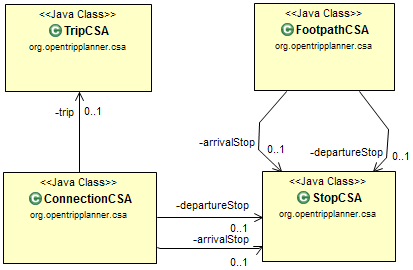
\includegraphics[width=8cm]{img/UML-TimeTable.png}
	\caption{Hier ist das UML-Diagramm zur TimeTable Datenstruktur zu sehen.}
	\label{fig:uml-timetable}
\end{figure}

\subsubsection{FootpathCSA}
\begin{figure}[htb]
	\centering
	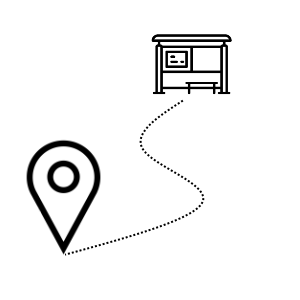
\includegraphics[width=5cm]{img/footpath.png}
	\caption{Symbolbild für den Fussweg(FootpathCSA)}
	\label{fig:footpath}
\end{figure}
Ein Footpath kann zwei verschiedene Funktionen haben. Er besteht aus einem DepartureStop, einem ArrivalStop sowie einer Dauer. Wenn der DepartureStop und der ArrivalStop gleich sind repräsentiert der Footpath einen Umsteigeprozess. Wenn sie unterschiedlich sind repräsentiert er einen Laufweg zu einem Stop hin oder von einem Stop weg.


\subsubsection{StopCSA}
\begin{figure}[htb]
	\centering
	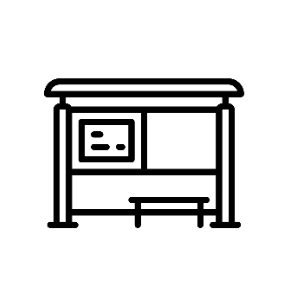
\includegraphics[width=5cm]{img/stop.png}
	\caption{Symbolbild für die Haltestelle(StopCSA)}
	\label{fig:stop}
\end{figure}
Ein Stop ist eine Haltestelle für öffentliche Verkehrsmittel. Ein Stop besitzt einen Namen, Längen- und Breitengrad. 

\subsubsection{ConnectionCSA}
\begin{figure}[htb]
	\centering
	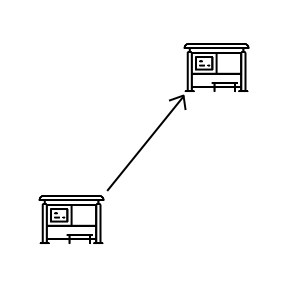
\includegraphics[width=5cm]{img/connection.png}
	\caption{Symbolbild für die Verbindung(ConnectionCSA)}
	\label{fig:connection}
\end{figure}
Eine Connection ist eine Verbindung zwischen einem DepartureStop und einem ArrivalStop . Die Connection hält Daten wie die Abfahrtszeit vom DepartureStop und die Ankunftszeit vom ArrivalStop. Zudem weiss die Connection zu welchem Trip sie gehört. Sie besitzt auch eine CompareFunktion (Vergleichsfunktion) um sich in einer Liste einzuordnen z.B. nach der Abfahrtszeit.

\subsubsection{TripCSA}
\begin{figure}[htb]
	\centering
	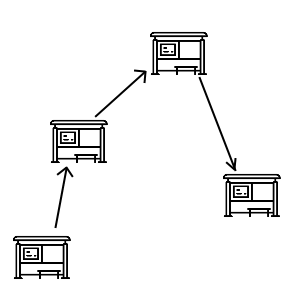
\includegraphics[width=5cm]{img/trip.png}
	\caption{Symbolbild für die Fahrt(TripCSA)}
	\label{fig:trip}
\end{figure}
Als Trip wird die Fahrt eines Öffentlichen-Verkehrsmittels von der Start-Station bis zur End-Station bezeichnet. Es ermöglicht den CSA ohne umsteigen erreichbare Orte zu erkennen. Ein Trip besteht aus mehreren Connections die aneinandergereiht sind. Desweiteren hält der Trip Informationen über das Verkehrsmittel(Zug,Bus usw.) und welche Geschäftsorganisation dieses Verkehrsmittel zur Verfügung stellt. Ausserdem enthält der Trip Informationen ob der Trip an jenem Tag auch fährt oder nicht.

\subsubsection{Journey}
Ein Journey ist ein vom CSA berechneter Weg vom Start- zum Zielpunkt. Er besteht aus einem StartPath, welcher den Fussweg zur ersten Station hin darstellt, sowie eine Liste aus journeyPointern welche den Weg mit allen Umsteigestationen repräsentiert. Neben den Gettern und Settern gibt es eine Klonfunktion. Für die Liste der journeyPointer gibt es Add-Funktionen zum Einfügen am Anfang, am Ende oder an einem bestimmten Punkt anhand eines Indexes.

\subsubsection{JourneyPointer}
Ein JourneyPointer ist eine Hilfskonstruktion welche der CSA anlegt um die berechnete Abfolge von Stationen später wieder rekonstruieren zu können.Ein JourneyPointer besteht aus einem Leg sowie einem Footpath. Dabei handelt es sich beim Leg um eine Fahrt in einem ÖV vom einsteigen bis zum Aussteigen und beim Footpath um das darauffolgende Umsteigen oder das erreichen des Ziels.

\subsubsection{LegCSA}
Ein Leg ist die Fahrt in einem Öffentlichen Verkehrsmittel vom einsteigen bis zum aussteigen. Dies ermöglicht es den Journey nicht von Station zu Station, sondern von Umsteigen zu Umsteigen zu rekonstruieren. Ein Leg besteht aus einer EnterConnection und einer ExitConnection. Er besitzt neben den Gettern, Settern und Konstruktoren keine weiteren Methoden.

\subsection{Programmablauf}
\begin{figure}[htb]
	\centering
	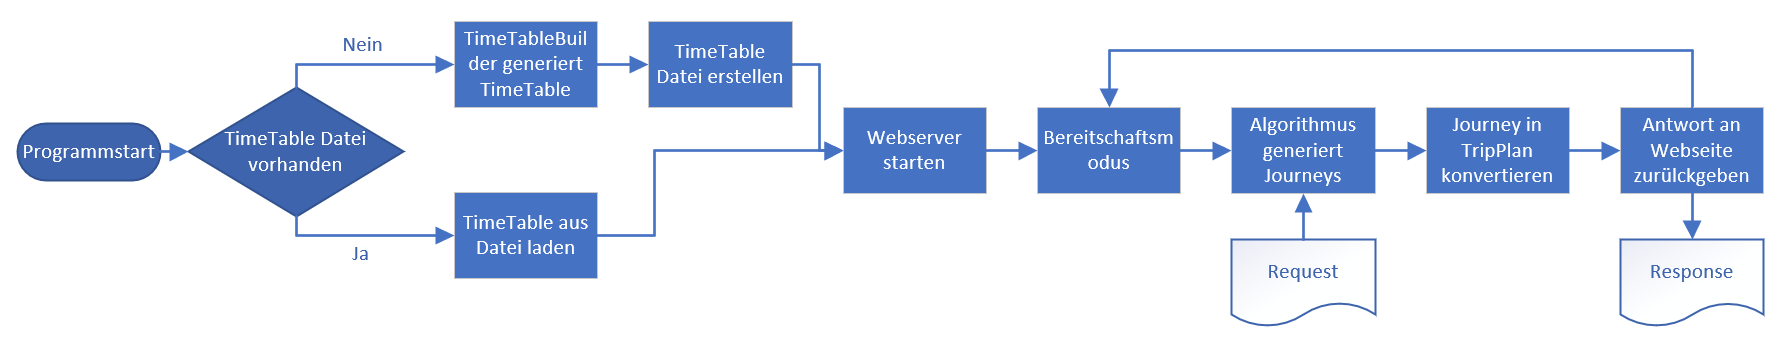
\includegraphics[width=15cm]{img/programmablauf.png}
	\caption{Programmablauf des OTP mit dem CSA}
	\label{fig:programmablauf}
\end{figure}

\subsubsection{TimeTableBuilder}
Da wir für den CSA eine Zeittafel(TimeTable) benötigen, muss diese durch den Zeittafelersteller (TimeTableBuilder) erstellt werden. Die zugrundeliegenden GTFS-Daten können jedoch nicht in dieser Form einfach der Zeittafel übergeben werden. Der Zeittafelersteller erzeugt die Zeittafel. Durch die Funktion \texttt{.loadFromGtfs()} werden die Daten eingelesen und in die benötigte Form gebracht. Dieser Prozess kann durchaus einige Zeit in Anspruch nehmen. Deshalb wird nachdem die Zeittafel fertig befüllt wurde anschliessend serialisiert und als Java-SerializedObjectFile gespeichert. Somit brauchen wir nicht mehr jedesmal die Zeittafel komplett neu einzulesen und zu erstellen. Durch die Funktion \texttt{.loadFromSerializedObjectFile()} kann die zwischengespeicherte Zeittafel jederzeit eingelesen werden, was die Zeit um eine schon in Form gebrachte Zeittafel zu erzeugen um einiges verkürzt. Unabhängig von beiden Methoden wird dann der Server gestartet.

\subsubsection{Server}
\todocomment{Startet server welchen die Webseite für afrufe zur verfügung stellt}
\subsubsection{Webseitenaufruf}
Wenn ein Aufruf von der Webseite eingeht so wird die plan Methode der Klasse PlannerResource aufgerufen. Diese erhält die Anfragenparameter in einem RoutingRequest-Objekt. Das im Preprocessing generierte TimeTable-Objekt wird als neue Instanz übergeben. Dies wird gemacht, da der OTP eine seperate Isntanz des Algorithmusses für jeden Aufruf verwendet. Der TimeTable sowie der Request werden dann der createJourneys-Methode des Algorithmuses übergeben. Dessen Rückgabe wird in einem Set von Journeys gespeichert.

\subsubsection{Connection Scan Algorithm}
Der Connection Scan Algorithm, kurz CSA,  ist ein moderner Algorithmus zur Bearbeitung von Anfragen auf zeitplanbasierten Sytemen. Er basiert, im Gegensatz zu den gängigen Algorithmen wie z.B. dem Dijkstra-Algorithmus, nicht auf einem gewichteten Graphen. 
Es gibt zwei Arten des CSA. Zum einen den EACS(EarlyestArrivalConnectionScan) welcher die frühestmögliche Ankunftszeit und wenn benötigt auch noch den dazugehörigen Journey zurückliefert. Zum anderen den PCS(ProfileConnectionScan) welcher alle möglichen Journeys berechnet und den Bessten Journey nach mehreren Kriterien sortieren kann. Beide sind darauf ausgelegt genau einen Journey zurückzugeben.

\subsubsection{Earliest Arrival Connection Scan}
Der Earliest Arrival Connection Scan Algorithmus, kurz EACS, arbeitet mit einer nach Abfahrtszeit sortierten Liste von Verbindungen. Über diese iteriert er dann aufsteigend wobei als Startpunkt die erste Verbindung, welche nach der im Request spezifizierten Abfahrtszeit abfährt. 

Jede Verbindung wird auf drei Eigenschaften überprüft:
\begin{itemize}
	\item Ist der Abfahrtsort der Startort?
	\item Wurde der Abfahrtsort schon von einer früheren Verbindung erreicht?
	\item Wurde das zur Verbindung gehörende Fahrzeug schon von einer früheren Verbindung benutzt?
\end{itemize}
Wenn eine dieser drei Bedingungen erfüllt ist so wird dies im Ankunftsort der Verbindung mit einem Zeiger auf den Ort, bei welchem man in das jeweilige ÖV eingestiegen ist, vermerkt. Der Ort bei welchem man eingestiegen wird mithilfe eines Trip-Bits gespeichert. Wenn eine ÖV zum ersten mal verwendet wird so wird der Startort gespeichert und das Trip-Bit wird für das ÖV gesetzt. Wird das ÖV erneut verwendet so ist das Trip-Bit bereits gesetzt und der Startort wird nicht überschreiben. 

Sobald der Algorithmus eine Verbindung findet, welche eine der drei Bedingungen erfüllt und gleichzeitig der Ankunftsort dem Zielort entspricht, hat er einen Journey zum Ziel gefunden. Die Schleife wird unterbrochen und der Algorithmus baut sich vom Zielort aus mithilfe der Zeiger den kompletten Journey auf welcher dann als Antwort zurückgegeben wird.

Der ECSA existiert auch in einer schlankeren Version bei welcher keine Zeiger gespeichert werden. Dies führt dazu, dass der ECSA schneller ist, jedoch liefert er nur noch die Ankunftszeit ohne den Reiseweg zurück.

\subsubsection{Profile Connection Scan}
Der Profile Connection Scan Algorithmus, kurz PCS, arbeitet auch mit einer nach Abfahrtszeiten sortierten Liste von Verbindungen. Im Gegensatz zum EACS iteriert er absteigend über die Verbindungen. Er sucht als o die Verbindung vom Zielpunkt aus. Jede Verbindung durchläuft dabei drei Prüfungen:

\begin{itemize}
	\item Kommt man ans Ziel wenn man aussteigt?
	
	Diese Bedingung überprüft ob der Ankunftsort der Verbindung der Zielort ist. Sollte dies der Fall sein so wird im Abfahrtsort der Verbindung die Ankunftszeit sowie die dazugehörige Verbindung gespeichert. Zusätzlich wird die Ankunftszeit für das jeweilige ÖV gespeichert.
	\item Kommt man ans Ziel wenn man umsteigt?
	
	Es wird überprüft ob vom Ankunftsort der Verbindung schon ein Weg gefunden wurde, welcher zum Zielort führt. Dazu wird vom wird überprüft, ob im Ankunftsort eine Ankunftszeit gespeichert wurde. Ist dies der Fall so wurde schon ein möglicher Weg vom Ankunftsort zum Zielort gefunden. Dann werden die Informationen wie in der ersten Bedingung in Abfahrtsort und dem ÖV gespeichert.
	\item Kommt man ans Ziel wenn man sitzen bleibt?
	
	Es wird überprüft, ob von diesem ÖV aus schon eine Weg zum Zielort gefunden wurde. Dazu wird überprüft ob für das ÖV schon eine Ankunftszeit gespeichert wurde. Ist dies der fall so werden die Informationen wie in den ersten beiden Schritten im Abfahrtsort und dem ÖV gespeichert.
\end{itemize}
Die Suche ist abgeschlossen sobald die Abfahrtszeit der Verbindung früher als die im Request definierte Abfahrtszeit ist. 

Nun wird vom Startpunkt aus jede gespeicherte Ankunftszeit überprüft. Dann wird von der zur Ankunftszeit gehörigen Verbindung der Ankunftsort genommen. Von diesem Ort aus werden wieder die gespeicherten Ankunftszeiten überprüft und die gleichen Schritte erneut durchgeführt. Dies wird so lange wiederholt bis der Ankunftsort der Zielort ist. Der gefundene Weg entspricht dann einem Journey zum Ziel. Der beste gefundene Journey kann dann als Response zurückgegeben werden. 
\subsubsection{JourneyToTripPlanConverter}
Die vom Algorithmus gefundenen Journeys werden dann zusammen mit dem Request der generatePlan-Methode des JourneyToTripPlanConverter übergeben. Dieser wandelt die Journeys in ein TripPlan-Objekt um, welches von der Webapplikation als response erwartet wird.
Die vom Request benötigten informationen werden zu beginn in das TripPlan-Objekt übertragen. Danach wird aus jedem Journey ein Itinerary-Objekt erzeugt. Dieses wird dann mithilfe der dem Journey zugehörigen JourneyPointer befüllt. Für die Legs sowie die Footpaths der JourneyPointer wird ein Leg generiert. Dies ist jedoch ein Leg-Objekt und kein LegCSA-Objekt. Während des ersten durchlaufs wird zudem aus dem StartPath des Journeys ein Leg generiert. Dazu gibt es die beiden Methoden legFromLeg() und legFromFootpath(). Diese übertragen die benötigten Parameter und erstellen eine Geometrische-Form welche dem Fahrtweg folgen und für die Anzeige auf der Webseite benötigt werden. Wenn ein Leg aus einem Footpath generiert wird, wird zusätzlich überprüft ob dieser eine Distanz überwindet oder ob der Start- und Zielpunkt gleich sind. Dies dient dazu umsteigewege hinauszufiltern, welche von der Webseite nicht als Leg benötigt werden, jedoch trotzdem in die Zeit mit einfliessen. Sobald alle JourneyPointer abgearbeitet sind wird das Itinerary den TripPlan hinzugefügt. Nachdem die 3 besten Journeys konvertiert wurden wird der TripPlan an die Webseite zurückgegeben.
